\documentclass[envcountsame]{llncs}
\usepackage{amsmath,amsfonts}
\usepackage{lscape}
\usepackage{bm}
\usepackage{listings}
\usepackage[bookmarks,colorlinks,urlcolor=blue,citecolor=blue,linkcolor=blue]{hyperref}
\usepackage{graphicx}
\usepackage[utf8]{inputenc}

\DeclareBoldMathCommand{\t}{t}
\DeclareMathOperator{\loss}{\ell}
\newcommand{\segs}{\mathbb S}
\newcommand{\head}{\mathcal H}
\newcommand{\tail}{\mathcal T}
\newcommand{\best}{\mathcal V}

\usepackage[numbered,autolinebreaks,useliterate]{mcode}


%\newcommand{\mynote}[1]{\marginpar{\tiny #1}}
\newcommand{\mynote}[1]{}

\hypersetup{
	pdfauthor={Tim Scarfe},
	pdftitle={Notes on Sleeping Expert Regions Work},
pdfkeywords={},
pdfsubject={},
pdfcreator={Tim Scarfe},
pdfproducer={Tim Scarfe},
}


\institute{Computer Learning Research
 Centre and Department of Computer Science, \\ 
Royal Holloway,  University of London, Egham, Surrey, TW20 0EX, United Kingdom\\
\email{tim@cs.rhul.ac.uk}}

\title{
Notes on Sleeping Expert Regions Work}
\author{Tim Scarfe}

\begin{document}

\maketitle

\begin{abstract}
Notes on Sleeping Expert Regions Work
\end{abstract}

\section{Sleeping Expert Regions}

First thing I did was make the regions overlapping, well at least with the capability to overlap if we want them to. 

In principle I have shown that regions exist (see figure \ref{fig:regionsexist}), and are contiguous and repeating in much the same way as the music work, so there is a chequerboard pattern visible. I was not able to demonstrate this previously so it lends credibility to the idea that old information can be useful. I can show the chequerboard using the loss matrix and the expert weights with the caveat that I need to use log scaling to see it. This makes sense on the expert weights because they get normalized by expert+1 as time goes on. This makes less sense for the loss matrix. 

Another concept is that in order to switch to the old regions and see the pattern you need a high alpha value which would obviously kill the performance of the algorithm. Catch 22. 

I can demonstrate that it's possible to get strong results purely tracing the matrix and avoiding the overheard of fixed share which is very naive anyway i.e. it just does a random fan out on all the experts looking for ones that happen to perform well. An improved scheme would be switching into the vicinity of another expert which is already making strong predictions assuming some contiguity exists (which it does). Even so I think we would still fail to perform well.

\subsection{What happens when no regions == no examples?}

This was the main intention for doing overlapping windows because of course this should be comparable in some sense to the online version. Assuming it switched to the new one every time (alpha=1) 

\section{Work Needed for Thesis}

I first need to demonstrate that we can trace this matrix and outperform the competitor with N switches. 

Then we need to construct an argument that a switching scheme exists that could leverage the region structure of the dataset. Perhaps we don't even need to do that, we can simply say that, say 17 switches could have worked, but with the corresponding alpha value; the overhead of the naive FS algorithm takes us ... brain melt. 

Fixed share is supposed to be a deterministic algorithm, so i don't really understand the random element to it. Fixed share has a very low loss (regret -- in comparison to the best switching expert sequence) which is linear in its parameters so why would we even bother coming up with another scheme?

\section{General Idea -- Experts could be time synced}

Might allow for slower switching.

It's clear from observation that time resolution is critical. We could have all experts rendering real time predictions but with varying parameters. I am mainly thinking about window size here to capture the regionalism through the visualization of the weights. Of course this could be combined with the experts of the main algorithm but if the latter wasn't a significant contribution it would probably have to be omitted from the work. 

Another cool idea is lagged experts, i.e. have experts that were trained for a fixed but tracking period in the PAST. 

After implementing this, I discovered that mixing window sizes does yield an improvement in performance but the weights don't tell an interesting story (see figure \cite{fig:mixregionsize}). 


\section{Yuri Meeting 2808 (18:30->20:15)}

\begin{itemize}
\item Big narrative idea we came up with was that we are talking about old information in the regions work and can demonstrate that using old information we can do nearly as well as new information using complicated models but probably the conclusions is that for volatility new information always rules but not for the reasons you think. It's more to do with the fact that parsimonious models built on new information are more adaptable (increased time resolution). Hmm. But then we would need to demonstrate that parsimonious models on old data wouldn't work well on new data. Actually they would. Brain melt. We should do a jerked ARIMA on the dataset for comparison. 
\item It could be hailed as a discovery that we have observed the contigous repeating regionality in the voilatility dataset at all. And yuri comments that there should be no regionality to price, it may just be a volatility thing. 
\item We observed this regionalityu and tried to design an algorithm to exploit it
\item Interesting then that the regions algorithm seems to pay a cost on the transition between regions, perhaps amplified by the number of experts that have weight on the old region that need to be shifted to new experts in the new region
\item Which brings us onto the new idea, time shifting regions that are syncronised with the online time of the algorithm, this should emlimitate some of the burden we pay for switching (no it wouldnt though)
\item Played with ridge, having the last volatility in signal doesnt actually improve, nor does clamping volatility to 1, check this. Seems we almost track the competitor 1:1 now, compare with arima

\end{itemize}

\subsection{Hit-List for tonight}

\begin{itemize}
\item Get these lagged experts working,they are the last hope
\item also try mixing in a zero lag expert and potentially fixed region experts
\item Might be worth mixing parameters but then it gets very arbitrary
\item Start writing this section up in the thesis
\item It's ok to just use the three volatility datasets
\item Describe the discovery of regionality in the three volatility datasets
\item Come up with e coherent explanation exactly why we fail even with experts==records, why is it so different to sliding, what about tweaking the introduction weight, presumably as it tends to 1 our performance tends to online ridge regression
\end{itemize}

\subsection{Night work notes}

\begin{itemize}
\item Feeling a bit tired tonight, starting at 01:22
\item I have just been going through some previous work, and in 2012 I was spending a lot of time working with ARIMA. I am trying to remember where the research went with that. I remember that we were trying to extend some results on Mishas thesis and it turned out that his work was flawed and that the network traffic dataset was essentially unpredictable. What I don't think we did properly was examine ARIMA on the russian datasets.
\item In particular we had an idea of enumerating parameters for the AR MA and allowing the prediction with expert advice algorithm select the best sets of parameters in an online fashion. Perhaps this will work on the russian data when it failed on the other. We need to dig this work up.
\item as a starter for ten we should test arima on the russian sets with jerking models and see how it performs in relation to ridge regression
\item need to figure out how to trace through the loss matrix, this will become part of our key argument about why fixed share does not work	
\end{itemize}


\begin{figure}
\centering
%\includegraphics[width=0.45\textwidth]{simmat_preds1.pdf}
%\hspace{1em}
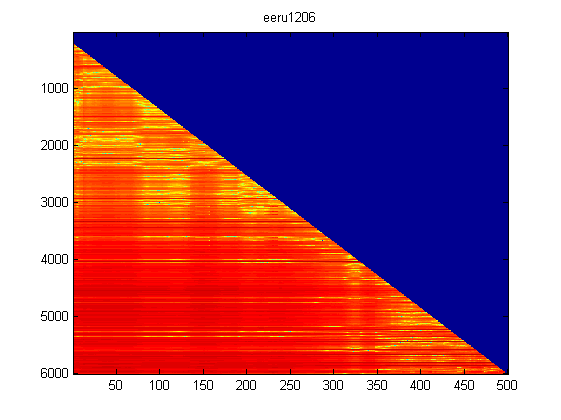
\includegraphics[width=0.8\textwidth]{images/reallareregions}
\caption{Hopefully a clear demonstration that repeating regions do exist in the dataset}
\label{fig:regionsexist}
\end{figure} 

\begin{figure}
\centering
%\includegraphics[width=0.45\textwidth]{simmat_preds1.pdf}
%\hspace{1em}
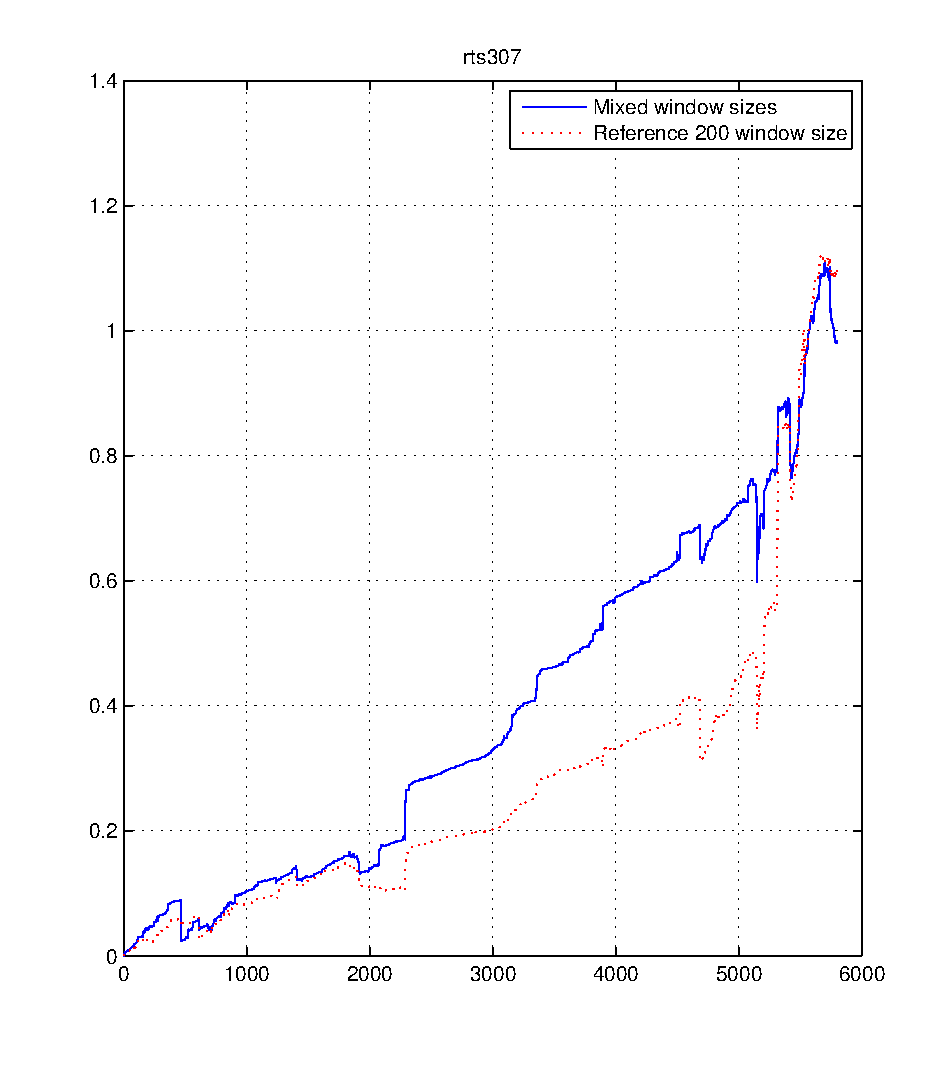
\includegraphics[width=0.8\textwidth]{images/mixed_regionsizes}
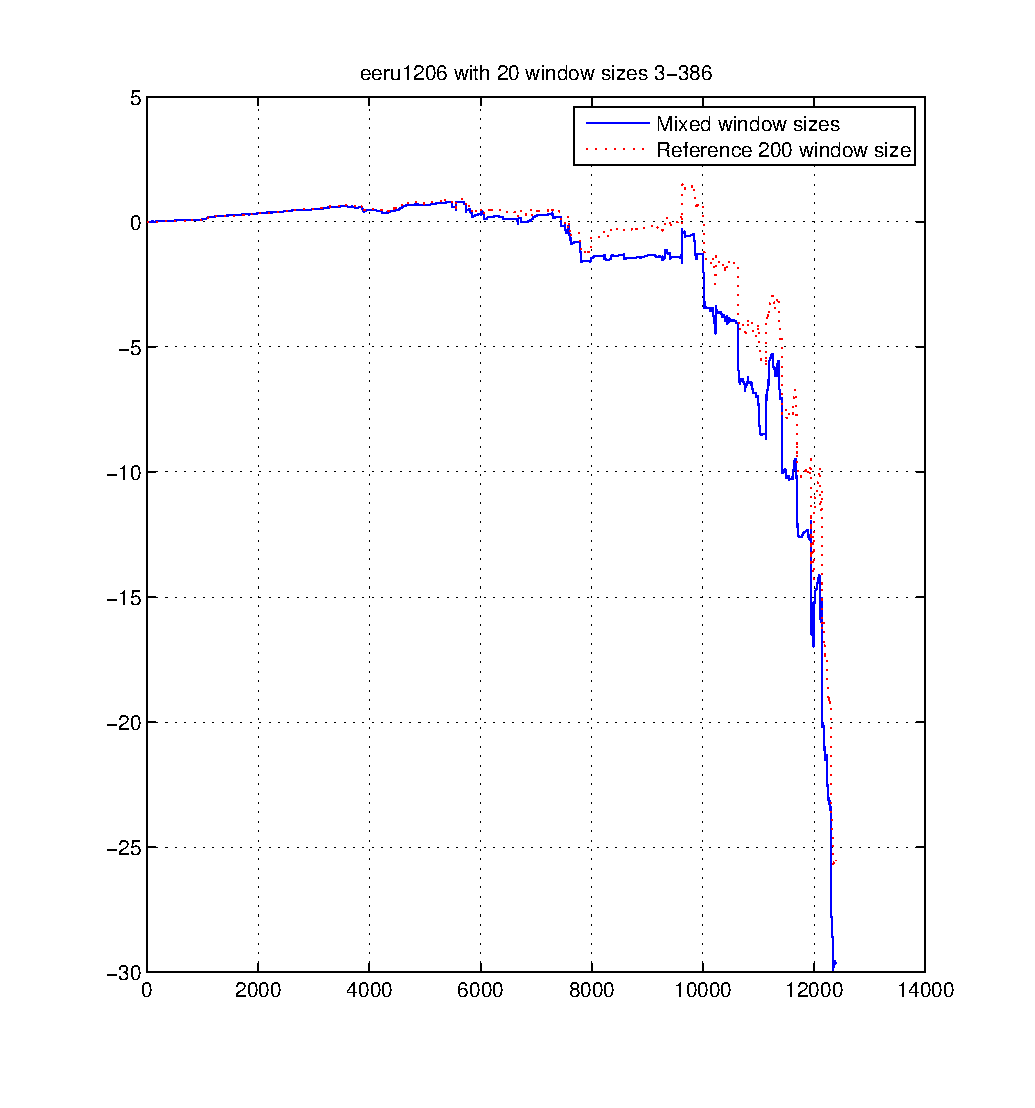
\includegraphics[width=0.8\textwidth]{images/mixed_regionsizes_eeru1206}
\caption{This is when we mix different window sizes (10 sizes from 10 to 500), the improvement is clear but the weights don't tell an interesting story}
\label{fig:mixregionsize}
\end{figure}


\section{Work Session 04 Sept}

Big idea. Just now thinking about a cool new idea. The thought process was some sort of comparison between sliding window ridge regression and the corresponding specialist expert algorithm.

The overhead is a killer. Because the new expert will always be the best but have no weight. Of course all the overhead comes from the fact that the experts are not time synced. So what if we time synced them?! This should look like the latest expert has all the weight, but if we see other regionality in the weights graph it suddenly gets fascinating!!

Wasted a lot of time being an idiot.

When I got it working, switching over it provided no improvement at all apart from near the end. This is still a discovery though isnt it. At the end of the dataset the benefit of the algorithm outweighs the overhead. Perhaps this has got some mileage on it see figure (\ref{fig:mixsliding}). 

Mixing different window sizes does help, perhaps there is some interaction between lag and window size. Tried some smaller window sizes that didnt work either.
	
Now looking back on the different window sizes. 

ARIMA we haven't looked at that yet.
What about mixing between using lag1,2,3,4,5 as the new prediction?!


\section{Work Session 06 Sept}

Starting at midday

I am thinking now that I need to pretty much run the experiments and start the write up. The glaring omission is some kind of time series experiments -- for example: 

\begin{itemize}
\item Sliding ARIMA for comparison -- perhaps this needs to be added on the current experiments as a comparator. Would it make us look ever weaker if it outperforms the competitor right from the get-go. I think it possibly would. 
\item Some kind of regions implementation using time series models
\item A really good thing to document would have been the random generation of coefficients for time series models then using PWEA to switch between them. I just had an idea now that you could train a model and get some coefficients then introduce new experts with drifting coefficients. If they get weight we stick with them otherwise we discard them. 
\end{itemize}

The arima issue is a bit of a blocking issue because we would need to incorporate it into any results that we do.

What is the structure of the mysterious second section that we are going to add to the thesis. 

\begin{itemize} 
\item Description of datasets
\item Discovery of time structure in datasets
\item Sliding window ridge regression and results of that, parameter selection etc
\item introduction of prediction with expert advice
\item introduction of specialist experts/ fixed share etc
\item Regions algorithm and the motivation for it
\item Lagged regions
\end{itemize}


\begin{figure}
\centering
%\includegraphics[width=0.45\textwidth]{simmat_preds1.pdf}
%\hspace{1em}
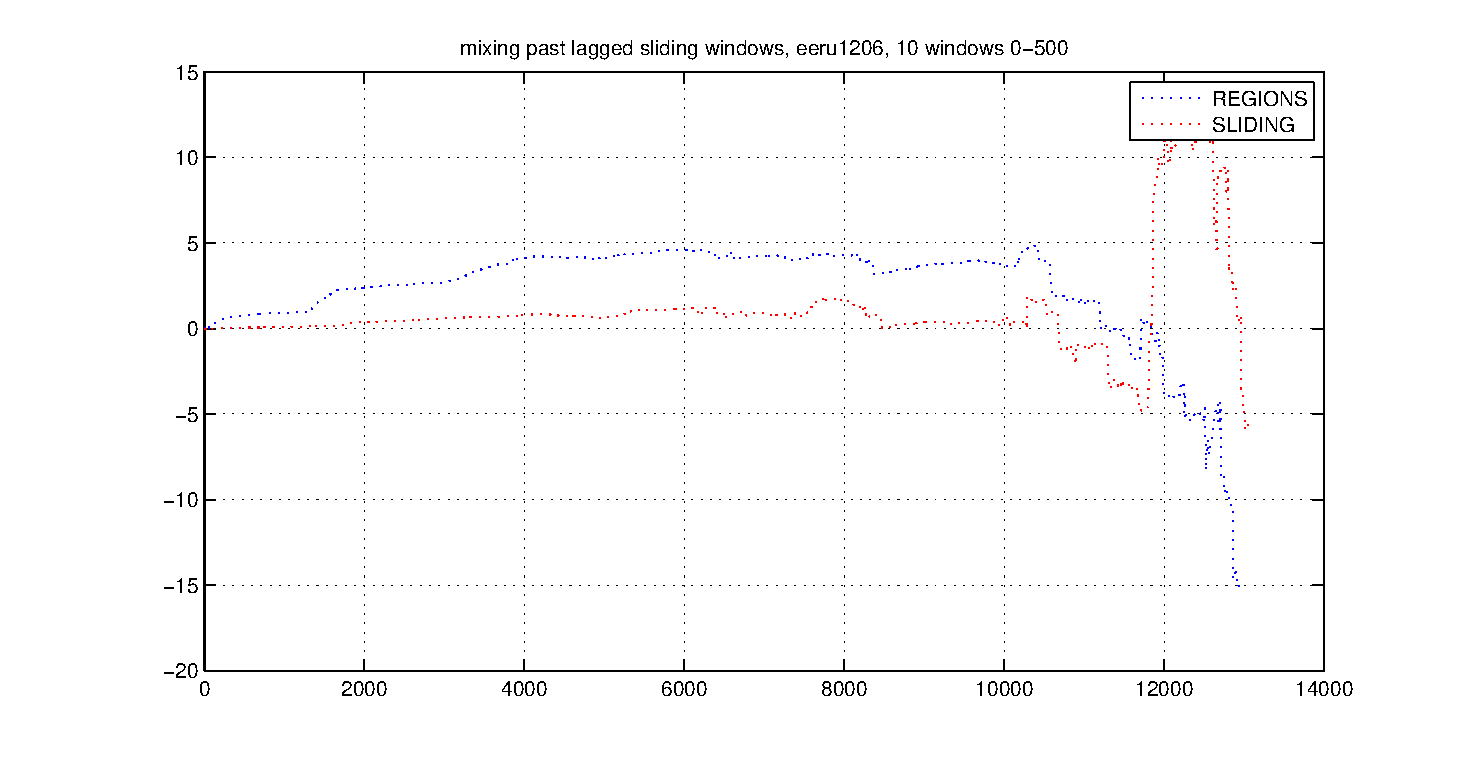
\includegraphics[width=0.8\textwidth]{images/mixed_sliding}
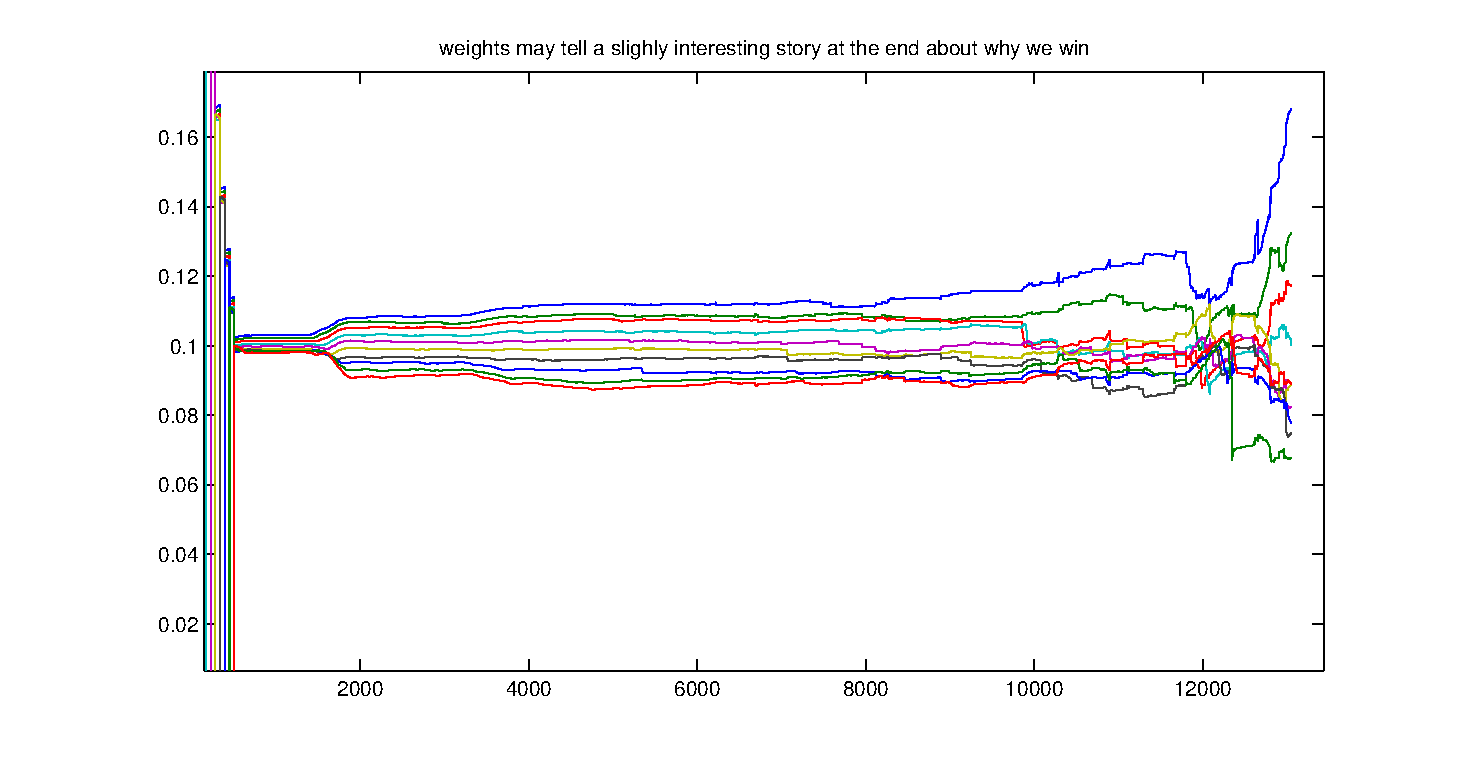
\includegraphics[width=0.8\textwidth]{images/mixed_sliding_weights}

\caption{So we can gain something on the end if we mix together sliding windows with different lags, these use windowsize of 100 with standard kernel settings}
\label{fig:mixsliding}
\end{figure}






\bibliographystyle{ieeetr}
\bibliography{references}

\end{document}
